%Made By Thomas Debelle
\documentclass{report}
\usepackage[a4paper, total={6in, 9in}]{geometry}
\usepackage[utf8]{inputenc}
\usepackage[francais]{babel}
\usepackage{graphicx}
\usepackage{graphics}
\usepackage[T1]{fontenc}
\usepackage{amsmath}
\usepackage{hyperref}
\usepackage{amssymb}
\usepackage{listings}
\usepackage{wrapfig}
\usepackage{xcolor}
\usepackage{array}
\usepackage{float}
\usepackage{amsfonts}
\usepackage{fancyhdr}
\usepackage{titlesec}
\usepackage{xparse}


\hypersetup{
    colorlinks=true,
    linkcolor=black,
    filecolor=magenta,
    urlcolor=cyan,
    pdftitle={Overleaf Example},
    pdfpagemode=FullScreen,
    }
\begin{document}


\begin{titlepage}
    \begin{figure}
        
\includegraphics[height = 2cm]{UCL_Logo.png}
        \label{fig:my_label}
    \end{figure}

    \hspace*{100cm}
    \centering
    \vspace*{7cm}

    {\Huge \textbf{Résumé de LINFO1104}}\\
    \vspace*{0.25cm}
    compilation du \today\\
    \vspace*{0.25cm}
    \Large{Thomas Debelle}\\

    \vspace*{9.5cm}
    {\Large Juin 2023}
\end{titlepage}


\tableofcontents
\newpage

\section*{Préface}

Bonjour à toi !\\

Cette synthèse recueille toutes les informations importantes données au cours, pendant les séances de tp et est amélioré grâce au note du Syllabus. Elle ne remplace pas le cours donc écoutez bien les conseils et potentielles astuces que les professeurs peuvent vous donner. Notre synthèse est plus une aide qui on l'espère vous sera à toutes et tous utiles.\\

Elle a été réalisée par toutes les personnes que tu vois mentionné. Si jamais cette synthèse a une faute, manque de précision, typo ou n'est pas à jour par rapport à la matière actuelle ou bien que tu veux simplement contribuer en y apportant ta connaissance ? Rien de plus simple ! Améliore la en te rendant \href{http://www.github.com/Tfloow/Q4_EPL}{ici} où tu trouveras toutes les infos pour mettre ce document à jour. (\textit{en plus tu auras ton nom en gros ici et sur la page du github})\\

Nous espérons que cette synthèse te sera utile d'une quelconque manière ! Bonne lecture et bonne étude.


\chapter{Introduction}
\section{Les Paradigmes}
Une paradigme, est une façon d'approcher et apporter une solution à un problème. De ce fait, chaque langage de programmation utilise 1 voir 2 paradigmes. Ce cours couvrat 5 paradigmes cruciaux qui sont:
\begin{enumerate}
\item "Functionnal Programming"
\item "Object Oriented Programming"
\item "Functional DataFlow Programming"
\item "Actor DataFlow Programming or Multi-Agent"
\item "Active Objects"
\end{enumerate}

Et pour découvrir ces paradigmes, nous utiliserons les langages de programmations \href{https://fr.wikipedia.org/wiki/Oz_(langage)}{"Oz"} qui est un langage de recherche multi paradigme ainsi que \href{https://fr.wikipedia.org/wiki/Erlang_(langage)}{"Erlang"}.

\chapter{Les différents Paradigmes}
Comme mentionner plus haut, on rencontrera 5 paradigmes dont voici le premier.
\section{Functional Programming}
Avec ce paradigme, on impose qu'une variable peut être nommé qu'une seule fois ! Donc: \quad X = 10 mais on ne peut pas plus loin dire X = 9. X est déjà attribué. On peut penser que cela risque d'être handicapant alors qu'en réalité, cela rend notre code plus simple à débugger. De plus, nombreux sont les langages et microservices utilisés qui implémentent la programmation fonctionnelle.
Formellement, quand on déclare une variable et qu'on l'assigne à une valeur ceci se passe.
\begin{wrapfigure}{r}{.4\textwidth}
	\centering
    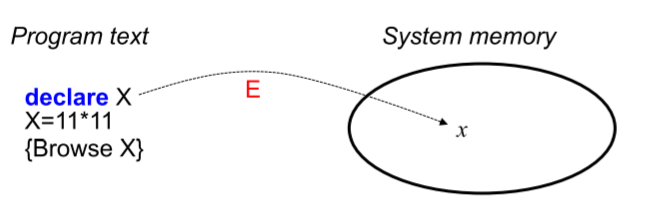
\includegraphics[width=.5\textwidth]{img/declVar.png}
    \caption{Déclaration d'une variable}
\end{wrapfigure}
Une chose importante à noter est que cette façon de programmer peut être réalisé dans n'importe quel langage de programmation. On peut également redéclarer un identificateur. C'est-à-dire écrire "X = 42" et plus loin en ayant redéclarer une variable "X = 11" car ces deux déclarations pointent à deux éléments totalement différents dans la mémoire.\\

Un "Scope" ou portée est une propriété centrale en programmation. En effet, c'est le scope qui nous permet d'avoir différente valeur pour des variables qui ont le même nom. Naturellement, elle ne représente pas la même chose car elle diffère de leur scope. On peut déterminer le scope d'une variable sans même exécuter le code. Il nous suffit d'analyser le code qui comprend un "\textcolor{red}{lexical scoping}" ou un "\textcolor{red}{static scoping}".
\begin{figure}[H]
\centering
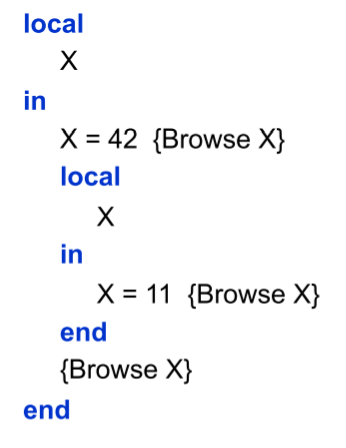
\includegraphics[width=3cm]{img/scope.png}
\caption{Exemple de code avec des scope différents}
\end{figure}
\section{Conseils pour la syntaxe d'Oz}

\chapter{Programmation symbolique}
\section{Listes}
On dit d'une liste est \textbf{récursive} si elle se définit par elle-même. C'est-à-dire elle fait appel à elle-même. On utilise la récursion pour les calculs et pour stocker des données.
Une liste est soit vide ou soit une pair \textit{d'une valeur suivi par une autre liste}. En \textbf{OZ} les variables, procédures et fonctions \textbf{doivent} commencer par une majuscule !
\subsection{Définition formelle}
En utilisant la notation \textbf{Extended Backus-Naur Form} ou \textit{EBNF} pour les intimes, on écrit une liste comme: <List T> ::= nil | T '|' <List T>. Une chose importante à noter est le deuxième "ou" qui s'écrit comme '|' signifiant qu'il n'appartient pas à la définition de List T mais plutôt à l'ensemble T '|' <List T>. Si on lit ceci, on dirait "\textit{Une list d'élément représentant T correspond à un élément vide ou un élément représentant T suivi d'une autre Liste d'élément T}.\\

\begin{wrapfigure}{r}{.4\textwidth}
	\centering
	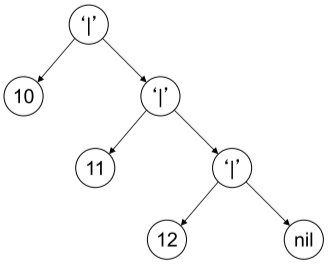
\includegraphics[width=.3\textwidth]{img/listTree.png}
\end{wrapfigure}
Donc une List d'entier se définit comme: <List <Int>
>. Une chose importante à remarquer est que j'ai utiliser le mot "représentation" en effet <Int> n'est pas un entier mais une représentation d'entier.\\

Pour définir une liste en Oz, on utilise soit la notation \textcolor{blue}{[1 2 3]} ou \textcolor{blue}{1 | 2 | 3 | nil}. C'est 2 déclarations reviennent à la même chose en mémoire. Une utilité des listes est leur facilité à être représenté sous forme d'arbre comme montré ci-contre.\\
En Oz, la \textit{head} est accessible via \textcolor{blue}{list.1} et la \textit{tail} est obtenu via \textcolor{blue}{list.2}.

\section{Pattern matching}
\begin{wrapfigure}{l}{.4\textwidth}
	\centering
	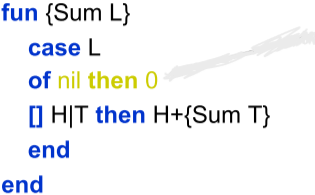
\includegraphics[width=.3\textwidth]{img/patternMatching.png}
\end{wrapfigure}
Grâce à cette représentation en arbre, il est plutôt aisé de voir si une liste est bien une liste ou si elle respecte une certaine structure définit par nos soins.\\
Ci-contre, on voit une fonction classique en Oz qui analyse une liste et détermine si elle est d'une structure correcte. Le \textcolor{blue}{[]} correspond au case où l'élément \textcolor{blue}{L} est une liste avec une Head et une Tail. On appelle cela une \textit{Clause} et H|T est le pattern de la clause. Le premier cas est définit par \textcolor{blue}{of}.

\section{Introduction au langage Kernel}
Le langage Kernel est la première partie de la sémantique formelle d'un langage de programmation. Une règle importante est que tout programme écrit en programmation fonctionelle \textit{peut être traduit en langage kernel}.
Les grands principes du langage Kernel sont:
\begin{itemize}
	\item Tous les résultats intermédiaires de calculs sont visibles.
	\item Toutes les fonctions deviennent des \textit{procédures} avec un argument en plus. Cet argument donne le résultat de la fonction.
	\item Les fonctions dans une fonction sont sortis de leur fonction et on leur donne un nouvel identificateur.
\end{itemize}
Les résultats de la traduction: Les programmes Kernel sont plus longs mais on voit facilement comment un programme s'exécute et on voit si il est \textit{tail-recursive}

\section{Les arbres}
Les arbres sont des structures de données extrêmement utiles et utilisées. On peut y stocker des données spécifiques, faire des calculs, ... Les arbres illustrent bien \textit{la programmation orienté but}. Par le standard \textit{EBNF}, on définit un arbre comme suit: <tree T> ::= leaf | t(T <tree T> ... <tree T>). Donc un arbre est une feuille ou \textit{leaf} qui est suivie par un ensemble de \textit{sous-arbres}. Les arbres sont forts similaires au liste si ce n'est que les listes n'ont qu'une sous-listes alors qu'un arbre peut avoir plusieurs sous-arbres.

\subsection{Ordered Binary tree}
Un arbre de ce type à 2 particularités:
\begin{itemize}
\item \textcolor{red}{Binary}: toutes les éléments hors les feuilles possèdes 2 sous-arbres.
\item \textcolor{red}{Ordered}: pour chaque arbre, la clé à gauche est plus petite que la clé de l'arbre et la clé à droite est plus grande.
\end{itemize}
Ce type d'arbre est très utile pour par exemple effectuer des recherches binaires et permet de facilement et rapidement trouver des données.

\subsubsection{Lookup K T}
Nous permet de trouver une valeur. Ce programme est plutôt simple et il nous suffit de regarder la clé de l'arbre où on est. Puis on compare avec notre recherche, si on est plus grand, on va à droite sinon à gauche. On répète le processus jusqu'à trouver la clé.\\
Lookup est très efficace car il s'exécute en \textcolor{red}{$log_2 n$}, le pire cas est si l'arbre n'est pas équilibré et il ressemble à une liste. Mais en général, en ayant un nombre suffisant de données, il est très rare d'avoir un arbre non équilibré.
\subsubsection{Insert K W T}
Il existe 4 possibilités.
\begin{enumerate}
\item remplace une feuille.
\item on remplace un noeud.
\item on remplace un sous-arbre à gauche.
\item on remplace un sous-arbre à droite.
\end{enumerate}
Le premier cas est le plus simple car on créé simplement un nouvel sous-arbre avec 2 feuilles. Si on remplace un noeud, on change la clé et la valeur du noeud.
Pour remplacer un sous-arbre, on garde les mêmes clés et valeur de Y pour le noeud mais on change le sous-arbre à gauche ou à droite en fonction.
\subsubsection{Delete K T}
Celle-ci est plus compliqué, on a 4 possibilités
\begin{enumerate}
\item La valeur qu'on veut supprimer n'existe pas
\item On supprime une feuille.
\item on supprime un sous-arbre à gauche.
\item on supprime un sous-arbre à droite.
\end{enumerate}
Voici.

\section{Tuples et Records}

\subsection{Tuples}
Un tuple est une manière de stocker des données de différents tuples, l'\textit{ordre} est \textit{important} dans un tuple. On doit également donné un nom, un \textbf{label}.
\begin{lstlisting}
X = state(1 b 2)
{Browse {Label X}}
{Browse {Width X}}
\end{lstlisting}
La première ligne défini un tuple ayant pour \textit{label} "state". La seconde ligne imprime le label du tuple. La dernière affiche sa taille. (c'est donc un entier toujours positif ou $0$)\\
Les champs dans les tuples sont numérotés de\textbf{ $1$ à width $X$}. On appelle aussi le champ (field) une "\textit{feature}". Un tuple possède toutes ces features de manière consécutives.\\

On peut donc ainsi construire des structures de données plus compliqués comme des arbres:
\begin{lstlisting}
declare
Y = left(1 2) Z = right(3 4)
X = mid(Y Z)
\end{lstlisting}

\begin{figure}[H]
\centering
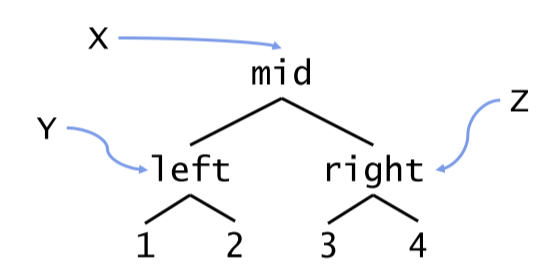
\includegraphics[width=5cm]{img/treeTuple.png}
\end{figure}
\subsubsection{Comparaison}
Il est très simple de comparer des tuples via "$==$", il ne faut simplement comparer leur value à chaque champ. Attention au \textit{loop} causé par les approches naïves.\\

\subsection{Similitude Tuples et liste}
En effet, une liste qui n'est autre que "H|T" peut facilement être traduit en tuple '|' (H T). Quand on peut déterminer un même élément via différentes manières, on appelle ça du \textit{sucre syntaxique}. Dans le \textit{kernel}, on fait au plus simple donc que des tuples.

\subsection{Les Records}
Les "\textit{records}" sont une \textbf{généralisation} des tuples. La différence avec les tuples est que le \textit{field} peut être n'importe quel valeur et ne doit pas être consécutif. Donc ceci est un \textit{record} correct:
\begin{lstlisting}
X = state(a:1 2:a b:2)
Y = inv(3:a 2:b 1:c)
\end{lstlisting}
Donc la position d'une valeur et son \textit{field} n'importe plus et on peut déclarer dans le sens qu'on veut.\\
Si on ne nomme pas un \textit{field} dans un \textit{record}, Oz va attribuer un nombre commençant à $1$ et qui n'est pas utilisé par un autre champ.\\
\subsection{Résumé}
\begin{itemize}
\item Un \textit{atom} est un record de width $0$.
\item Un tuple est un record avec des champs étant numéroté de manière consécutive de $1$ à width $X$. (consécutive, donc on skip pas. pas forcément dans l'ordre dans la déclaration)
\item Une liste est réalisé avec des \textit{tuples} et des $(X \quad Y)$
\item $\textbf{1}$ seule \textit{structure de donné} dans le kernel pour rester simple.
\end{itemize}

\section{Sémantique Formelle}
\subsection{Les environnements}
Un environnement est une fonction qui passe des \textit{identifieurs} aux \textit{variables en mémoire} autrement dit: $E_1 = {X \rightarrow x, Y \rightarrow y)}$

\subsubsection{Environnement contextuel}
Un \textit{environnement contextuel} d'une fonction contiens tous les \textit{identificateurs} qui sont usés dans la fonction mais déclaré \textit{en dehors}. Donc ce sont des fonctions qui lorsqu'on appelle une variable va pointer en dehors du scope de la fonction.

\subsubsection{Stocker une Procédure}
Les procédures sont stocker dans la mémoire sous le forme de procédure anonyme symboliser par le "\$".
\begin{lstlisting}
local P Q in
	{Browse 'do something'}
	proc {Q}
		{P}
	end
	{Browse 'another something'}
end
\end{lstlisting}
Notre "proc {Q}" sera stocker comme: "q = (proc\{\$\}\{P\} end, \{$P\rightarrow p$\})". On lit donc, la procédure \textit{anonyme} (\$), fais un appel à P (\{P\}) et fini (end), son \textit{environnement contextuel} fait que lorsqu'on appelle "P" on va récupérer la valeur "p" en mémoire (\{$P\rightarrow p$\}). Donc on voit que l'\textit{environnement contextuel} est stocker avec le code de procédure.\\
On appelle également la valeur d'une procédure une "\textit{closure}" ou une "\textit{lexically scoped closure}" car elle ferme les identificateurs libres quand défini.\\
Donc l'avantage d'un environnement contextuel nous permet d'être sûr qu'on appellera la bonne valeur même si elle est déclaré en dehors de la fonction.\\

Un \textit{identificateur libre} est un identificateur utilisé dans une \textit{fonction} qui est déclaré \textit{en dehors} de la fonction.\\
Les arguments d'une procédure \textbf{ne sont pas} des identificateurs libres car l'argument défini l'identificateur.

\subsection{Sémantique}
Il est important de comprendre le fonctionnement même d'un programme car si on ne comprend pas comme celui-ci fonctionne, il nous domine. \textit{If you do not understand something, then you do not master it – it masters you!}
\subsubsection{Définition}
La \textit{sémantique} d'un langage de programmation est une explication \textit{précise} de comment un programme s'exécute. Nous verrons la sémantique pour tous les paradigmes. Il en existe 4 types:
\begin{enumerate}
\item \textcolor{red}{Sémantique opérationnelle}: explique un programme sur base d'\textit{exécution} sur un PC simplifié appelé \textit{la machine abstraite}. $\rightarrow$ Fonctionne pour tous les paradigmes.
\item \textcolor{red}{Sémantique axiomatique}: explique un programme sur base d'\textit{implication}. C'est-à-dire que certaines \textit{propriétés} présent avant l'exécution, et d'autres seront présentes après. $\rightarrow$ très utilisé pour la programmation orienté objet comme \textit{Java}.
\item \textcolor{red}{Sémantique de notation}: explique un programme comme une \textit{fonction} sur un domaine abstrait. Donc simplifie l'analyse mathématique d'un programme. (utilisé dans \textit{Haskell} et \textit{Scheme})
\item \textcolor{red}{Sémantique logique}: explique un programme comme étant un \textit{modèle logique} basé sur des \textit{axiomes logiques}. Le résultat est une propriété correcte dérivé des axiomes. (cela est implémenté par exemple dans \textit{Prologue} ou dans la \textit{programmation sous contrainte})
\end{enumerate}

\subsection{Sémantique opérationnelle}
Ce type de sémantique à 2 parties majeures:
\begin{itemize}
\item \textcolor{red}{Langage Kernel}: traduit le programme en langage Kernel.
\item \textcolor{red}{Machine abstraite}: puis exécute le programme sur la machine abstraite.
\end{itemize}

\subsubsection{1. Langage Kernel complet}
Pour définir correctement une sémantique, il faut tout d'abord s'intéresser à son langage Kernel complet. On peut également prouver qu'un programme est correct en analysant son kernel. Par exemple, prenons ce code kernel:
\begin{lstlisting}
<s> ::= skip 
	| <s>1 <s>2 
	| local <x> in <s> end 
	| <x>1=<x>2 
	| <x>=<v> 
	| if <x> then <s>1 else <s>2 end 
	| {<x> <y>1 ... <y>n} 
	| case <x> of <p> then <s>1 else <s>2 end

<v> ::= <number> | <procedure> | <record>  
<number> ::= <int> | <float> 
<procedure> ::= proc {$ <x>1 ... <x>n} <s> end
<record>, <p> ::= <lit> | <lit>(<f>1:<x>1 ... <f>n:<x>n)
\end{lstlisting}
donc "<s>" contient le programme exécuté, "<v>" est une structure de donné contenant différent type de structure de donné qui sont définis juste en dessous. 

\subsubsection{2. La machine abstraite}
Voici ci-dessous comment s'exécute un programme initialement.

\begin{figure}[H]
\centering
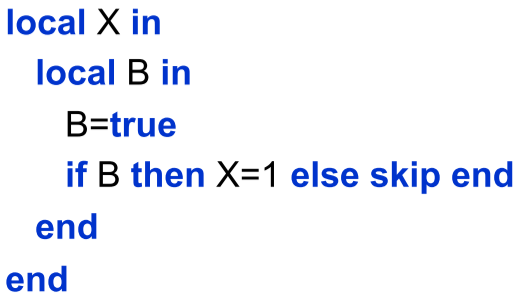
\includegraphics[width=5cm]{img/kernel.png}
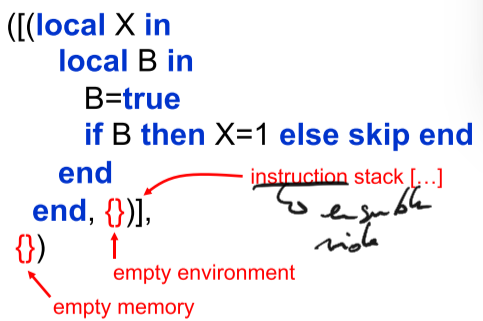
\includegraphics[width=5cm]{img/kernel1.png}
\caption{à gauche: programme écrit en Oz $\qquad$ à droite: état initiale d'exécution}
\end{figure}
Au début, l'environnement et la mémoire sont vides. L'état d'exécution est écrit typiquement comme:
\begin{lstlisting}
([(<s>,E)],sigma)
\end{lstlisting} %trouver comment utiliser un code dans lst
Sur la machine abstraite, on va d'instructions en instructions. C'est-à-dire on descend petit à petit.
donc on a pour la suite:
\begin{figure}[H]
\centering
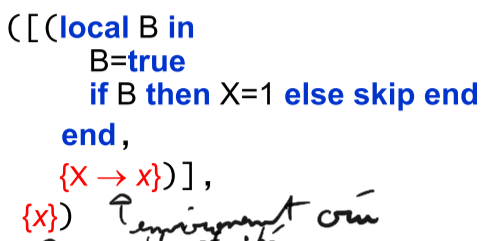
\includegraphics[width=5cm]{img/kernel2.png}
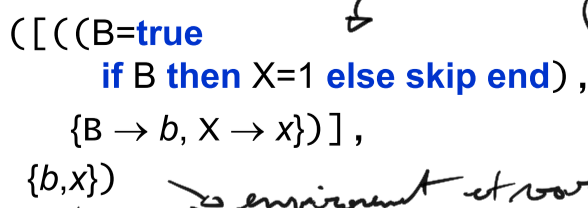
\includegraphics[width=5cm]{img/kernel3.png}
\caption{à gauche: on descend de 1 cran $\qquad$ à droite: on descend encore de 1 cran}
\end{figure}
On voit que au fur et à mesure qu'on descend, la pile de mémoire et d'environnement s'agrandit. Ensuite on va \textit{séparer} la \textit{composition séquentielle} comme suit:

\begin{figure}[H]
\centering
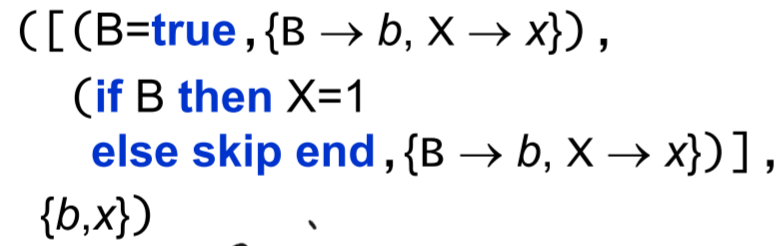
\includegraphics[width=5cm]{img/kernel4.png}
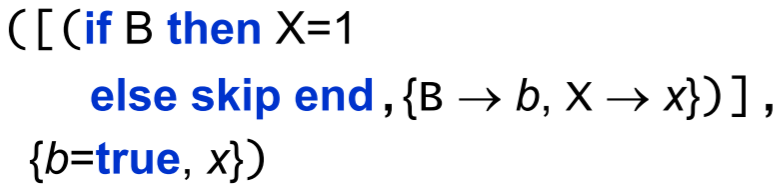
\includegraphics[width=5cm]{img/kernel5.png}
\caption{à gauche: on sépare en deux $\qquad$ à droite: on attribue à b la valeur définit à gauche}
\end{figure}
Une nouvelle instruction va s'ajouter à cause du "then" de notre condition:

\begin{figure}[H]
\centering
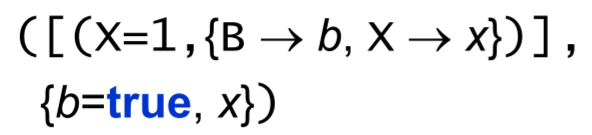
\includegraphics[width=5cm]{img/kernel6.png}
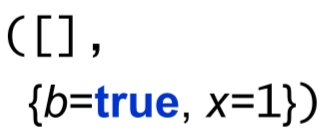
\includegraphics[width=3cm]{img/kernel7.png}
\caption{à gauche: la nouvelle instruction $\qquad$ à droite: les instructions sont vides, c'est fini}
\end{figure}

\subsubsection{3. Définir la machine abstraite}
\begin{itemize}
\item Pour chaque instructions dans le langage Kernel, on associe sa règle dans la machine abstraite
\item Chaque instructions prends un état d'exécution en entrée et sort un état d'exécution en sortie $\rightarrow (ST, \sigma)$.
\end{itemize}
L'instruction la plus simple est "\textcolor{blue}{skip}" car il fonctionne comme $([(skip, E), S_2, ..., S_n], \sigma)$ et renvoie $([S_2, S_n], \sigma)$ 

\begin{center}
\begin{tabular}{|c|c|c|}
\hline
Instructions & entrée & sortie\\
\hline
\textcolor{blue}{skip} & $1$ & $2$\\
\hline 
\textcolor{blue}{$(<s>_1 <s>_2)$} & $([(S_a S_b), S_2, ..., S_n], \sigma)$ & $([S_a, S_b, S_2, ..., S_n], \sigma)$\\
\hline 
\textcolor{blue}{local in <x> in <s> end} & $([(\text{local } <x> \text{ in } <s> \text{ end }, E)$ & $([(<s>, E+\{<x>\rightarrow x\})$\\
 & $, S_2, ..., S_n], \sigma)$ & $, S_2, ..., S_n], \sigma)$\\
\hline 
\end{tabular}
\end{center}
Il y a également d'autres types d'instructions dont on détaillera pas le langage en machine abstraite:

\begin{itemize}
\item \textcolor{blue}{<x>=<v> (crée et assigne une valuer)}: quand <v> est une procédure, on \textbf{doit} crée un environnement contextuel.
\item \textcolor{blue}{if <x> then <s>1 else <s>2 end (condition)} : si <x> n'est pas attribué, l'instruction va attendre (“\textit{block}”) jusqu'à ce que <x> soit attribuer à une valeur.
\item \textcolor{blue}{case <x> of <p> then <s>1 else <s>2 end} : Le system de "\textit{case}" se construit en combinant des structures de données Kernel.
\item \textcolor{blue}{\{<x> <y>1 ... <y>n\}} : ceci est la base de l'abstraction de donnée
\end{itemize}
Par ailleurs, voici d'autres concepts de machine abstraite:
\begin{itemize}
\item \textcolor{blue}{Single-assignment memory }\textcolor{red}{$s = \{x1=10,x2,x3=20\}$}: Définition d'une variable et la valeur associée.
\item \textcolor{blue}{Environnement }\textcolor{red}{$E = \{X \rightarrow x, Y \rightarrow y\}$}: Lien entre un identificateur et son lien dans la mémoire
\item \textcolor{blue}{Instruction sémantique }\textcolor{red}{$(<s>, E)$}: Une instruction avec son environnement.
\item \textcolor{blue}{Stack Sémantique }\textcolor{red}{$ST = [(<s>_1,E_1), ..., (<s>_n,E_n)]$}: Un stack d'instructions sémantiques.
\item \textcolor{blue}{État d'exécution }\textcolor{red}{$(ST,\sigma)$}: Une paire d'un stack sémantique et sa mémoire.
\item \textcolor{blue}{Execution }\textcolor{red}{$(ST_1,s_1) \rightarrow (ST_2,s_2) \rightarrow (ST_3,s_3) \rightarrow ...$}: Une séquence d'état d'exécution. 
\end{itemize}

\subsubsection{4. Programme correcte}
grâce à la sémantique, on sait prouver qu'un programme est correct. On dit qu'un programme produit une solution correcte, on l'appelle une \textit{spécification} et on voit qu'un programme est correct via la \textit{sémantique}.\\
Donc on prouve qu'un programme satisfait la \textit{spécification} quand on utilise une certaine \textit{sémantique}. La sémantique lie le \textit{programme} à un résultat mathématique appelé \textit{spécification}.\\

Donc on lie une vérité mathématique à un programme. Et on prouve cela via ces différentes étaps: (exemple avec une factorielle)

\begin{enumerate}
\item On commence avec la spécification du programme.
\item Notre programme est \textit{récursif} donc on va utiliser une preuve mathématique par \textit{induction}.
\item On doit prouver le cas de base et le cas général.
\item On utilise la sémantique pour prouver la véracité de notre programme.
\end{enumerate}

\subsubsection{5. Procédures}
Les procédures sont la base de toutes \textcolor{red}{abstractions de données}.\\
Il y a deux choses importantes dans une \textit{procédure}: sa \textcolor{red}{définition} et son \textcolor{red}{appel}.\\

\textcolor{red}{Définition}: on crée l'environnement \textit{contextuel}. Puis, on stocke le code de la procédure et son environnement.\\

\textcolor{red}{Appel}: on crée un nouvel environnement combinant l'environnement \textit{contextuel} de la procédure et les variables \textit{formelles}. Ensuite, le tout est exécuté.
\begin{lstlisting}
local Z in 
	Z=1
	proc{P X Y}Y=X+Z end
end
\end{lstlisting}
Ici, le seul identificateur \textit{libre} est \textbf{Z} qui est donc déclaré en dehors de la \textit{procédure}. Donc à l'exécution de \textbf{P}, \textbf{Z} est connu donc \textbf{Z} fait partie de l'environnement contextuel de la \textit{procédure}.
\begin{lstlisting}
local P in
	local Z in 
		Z=1
		proc{P X Y}Y=X+Z end
	end
	local A B in
		A=10
		{P A B}
		{Browse B}
	end
end 
\end{lstlisting}
Ici, à la ligne de la création de la procédure P, son environnement contextuel est $E_c = \{Z \rightarrow z\}$. Au moment de l'exécution de P avec les valeurs A et B, on va donc ajouter un environnement qui de la sorte: $E_P = \{Y \rightarrow b, X \rightarrow a, Z \rightarrow z\}$
Donc en langage \textit{sémantique}, la définition d'une procédure ressemble à cela:
\begin{itemize}
\item \textbf{Instruction sémantique}: (<x>=\textcolor{blue}{proc}\{\$ $<x>_1, ..., <x>_n$\} <s> \textcolor{blue}{end}, E)
\begin{itemize}
\item \textbf{Arguments formels}: $<x>_1, ..., <x>_n$
\item \textbf{Identificateurs libres de <s>}: $<z>_1, ..., <z>_k$
\item \textbf{Environnement contextuel}: $E_C = E_{|<z>_1, ...n <z>_k}$ (que les identificateurs libres)
\end{itemize}
\item Cela crée une liaison en mémoire de la forme: x(\textcolor{blue}{proc}$\{\$<x>_1, ..., <x>_n\}$<s>, \textcolor{blue}{end}, $E_C$)
\end{itemize}
Maintenant, voyons pour un \textit{appel sémantique}:
\begin{itemize}
\item \textbf{Instruction sémantique}: (\{$\langle x \rangle \langle y \rangle_1 ... \langle y \rangle_n$\}, E)
\begin{itemize}
\item Si la condition est \textit{false} donc $E(\langle x \rangle)$ n'est pas lié.
\item Si $E(\langle x \rangle)$ n'est \textbf{pas} une procédure, on a une erreur de \textit{condition}.
\item Si $E(\langle x \rangle)$ est une procédure \textit{mais} avec le mauvais nombre d'argument, on a aussi une erreur de \textit{condition}.
\end{itemize}
\end{itemize}
Une chose primordiale à comprendre est comment sont stocké les instructions. Elles sont stocké sur une \textbf{pile} (\textit{stack}). Donc on a l'instruction sémantique sur le stack: (\{$\langle x \rangle \langle y \rangle_1 ... \langle y \rangle_n$\}, E) avec la définition de procédure dans la \textit{mémoire} comme cela: $E(\langle x \rangle) = proc\{\$ \langle z \rangle_1, ..., \langle z \rangle_n\} \langle s \rangle \text{end}, E_c)$ \\
Ensuite, on met ces instructions sur la \textit{pile} $(\langle s \rangle , E_C + \{\langle z \rangle_1 \rightarrow E(\langle y \rangle_1), ..., \langle z \rangle_n \rightarrow E(\langle y \rangle_n)\})$\\

La machine abstraite fait 2 choses:
\begin{enumerate}
\item \textcolor{red}{Adjonction}: $E_2 = E_1+\{X \rightarrow y\}$ Donc ajoute une paire (identificateur $\rightarrow$ variable) à l'environnement. Ré-écrit par dessus $E_1$ si existe déjà. Utile pour \textcolor{blue}{local} $<x>$ \textcolor{blue}{in} $<s>$ \textcolor{blue}{end}.
\item \textcolor{red}{restriction}: $E_C = E_{|\{X,Y,Z\}}$ Donc limite les \textit{identificateurs} dans un environnement. On a besoin de cela pour calculer l'environnement \textit{contextuel}.
\end{enumerate}
Une adjonction:
\begin{lstlisting}[escapechar=\%]
local X in
	(E1) X=1 
	local X in 
		(E2) X=2 
		{Browse X}
	end 
end
E1 = {Browse %$\rightarrow$% b, X %$\rightarrow$% x}
E2 = E1 + {X %$\rightarrow$% y} = {Browse %$\rightarrow$% b, X %$\rightarrow$% y}
\end{lstlisting}
Une restriction:
\begin{lstlisting}[escapechar=\%]
local X in 
	(E1) X=1	
	local X in 
		(E2) X=2
		{Browse X}
	end
end
E1 = {Browse %$\rightarrow$% b, X %$\rightarrow$% x}
E2 = E1 + {X %$\rightarrow$% y} = {Browse %$\rightarrow$% b, X %$\rightarrow$% y}
\end{lstlisting}
\subsection{Résumé}
Définir la sémantique permet de relier les programmes au mathématique. On donne des instructions \textit{sémantique} au \textit{kernel} pour qu'il sache comment exécuter dans la \textit{machine abstraite}. La sémantique nous permet de prouver qu'un programme est \textit{correct}.\\
La sémantique est au cœur de la programmation. Une nouvelle librairie est comme si on ajoutait des instructions au programme donc on augmente sa sémantique.\\
Quand on écrit un programme, il faut comprendre la sémantique (l'utilisateur n'a pas besoin de savoir). La sémantique doit être simple et complète.\\
On peut voir la sémantique comme le langage de programmation \textit{ultime}.\\
Il ne faut pas oublier que les pc sont baser sur les mathématiques \textit{discrètes}.

\section{Rappel procédure sémantique}
Tout d'abord, en programmation nous avons différentes étapes qui reposent chacun sur les précédentes. Fermeture $\rightarrow$ Programmation d'ordre supérieur $\rightarrow$ Abstraction des données $\rightarrow$ Technologie de l'information.\\

Rappel sur l'exécution d'un programme:
\begin{lstlisting}
{Browse {Inc 10}}	#Langage pratique (classique)
local M in		 	#Langage Kernel
	local N in
		M=10
		{Inc M N}
		{Browse N}
	end
end
\end{lstlisting}
A l'exécution,$[(\{Inc M N\},\{M\rightarrow m,N \rightarrow n,Inc \rightarrow i,Browse \rightarrow b\}), (\{Browse N\},\{M \rightarrow m,N \rightarrow n,Inc \rightarrow i,Browse \rightarrow b\})],
\{m=10,n,i=(proc \{\$ X Y\} Y=X+A end, \{A \rightarrow a\}), a=1,b=(... browser code…)\}$ et Inc va référencer cela:\\
$[(Y=X+A,\{A\rightarrow,X \rightarrow m,Y \rightarrow n\}), (\{Browse N\},\{M \rightarrow m,N \rightarrow n,Inc \rightarrow i,Browse \rightarrow b\})],
\sigma$


\chapter{Programmation d'ordre supérieur}
Ce concept découle directement du concept d'\textit{environnement contextuel}. Dans un \textit{procédure} ou \textit{fonction} (les mêmes pour un langage kernel) peuvent prendre des valeurs ou des fonctions en arguments.
\subsubsection{Définition}
\begin{itemize}
\item Une fonction est dit \textcolor{red}{de premier ordre} si elle ne prend et ne ressort aucune fonction.
\item Une fonction est \textcolor{red}{N+1} si son entrée et sortie contiennent $N$ arguments.
\end{itemize}
Nomenclature des différentes fonctions:
\begin{itemize}
\item \textbf{Une génératrice} est le fait de prendre une fonction en entrée d'une fonction.
\item \textbf{Une instantiation} est le fait de retourner une fonction en sortie d'une fonction.
\item \textbf{Une composition de fonctions} est le fait de prendre 2 fonctions en entrée et on retourne leur composition.
\end{itemize}

\subsubsection{Utilisation}
Via la programmation d'ordre supérieure, on peut caché un accumulateur. On dit qu'on fait une \textit{abstraction d'accumulateur}.\\
Une fonction type est la fonction \textbf{FoldL} (\textit{reduce}). En effet, la fonction FoldL fait:
\begin{lstlisting}
declare
fun {FoldL L F U}
	case L
	of nil then U
	[] H|T then {FoldL T F {F U H}}
	end
end

{FoldL LIST Function Acc}
\end{lstlisting}
On peut, un peu dans le même style, faire de l'encapsulation afin de cacher sa valeur à l'intérieur. $\rightarrow$ C'est la base de \textit{l'abstraction de donnés}.\\

Il faut faire attention à l'\textbf{exécution retardé}. En effet, si on ne stocke pas le résultat d'une fonction, elle ne sera exécuté que quand on appellera la valeur. Donc cela peut prendre beaucoup de place en mémoire de stocker une fonction plutôt que son résultat.


\end{document}


